The general VSC problem as given in chapter~\ref{prelim} was first studied in \cite{gibbons} to test if shared memory multiprocessors provide a sequentially consistent memory. The problem is in general hard even with restrictions such as bounded threads, bounded variables or just one writer. Later Qadeer and Musuvathi \cite{musuvathi} showed that most  concurrency bugs can manifest within a few number of  preemptions. Also, bounding preemption decreases the state space exploration significantly. So a naural question is what happens to the complexity of the VSC-problem when number of  preemptions is fixed?
We study how the complexity varies across \onewriter{}, \twowriter{} and \threewriter{} programs and discuss the proofs of all the relevant theorems introduced in Chapter~\ref{prelim}.

\section{VSC under fixed preemptions}\label{VSCp}

Recall the VSC$^\pp$-problem from last chapter: given a concurrent program $\program$ and a fixed constant $\pp$, is there an interleaving of $\program$ containing at most $\pp$ preemptions which is sequentially consistent? 

The complexity for VSC$^\pp$ is polynomial for $\onewriter$ programs as given in the next section. The following sections show the hardness results for \twowriter{} and \threewriter{} programs.

\subsection{Results for Single Writer}

We intend to prove the following theorem. 
\begin{theorem}\label{th:onewriter} \vscp  admits a polynomial-time solution for \onewriter\ programs.  
\end{theorem}

For the rest of this section, fix a \onewriter\ program $\program$ with $k$ threads having a total of $n$ events across all threads, 
and a constant $\pp \geq 0$. Here is an overview of our algorithm. 
\begin{description}
\item[Step 1.] Guess a set $\points$ of at most $\pi$ events.
\item[Step 2.] Decide whether there exists an SC interleaving of $\program$ where the preemptions occur exactly after the events in $\points$.
\end{description}
Step 1 can be done in $\mathcal{O}(n^{\pp})$.  For Step 2, we present an algorithm that has complexity $\mathcal{O}(n^3 \cdot k^2 \cdot \pp \cdot \pp!)$.  Hence, the overall complexity  comes to $\mathcal{O}(n^{\pp + 3} \cdot k^2 \cdot \pp \cdot \pp!)$. Since $\pi$ is fixed, we get a polynomial-time algorithm for the \vscp\ problem for \onewriter\ programs. We now present our algorithm with examples.  

 \begin{figure}[t]
 \centering
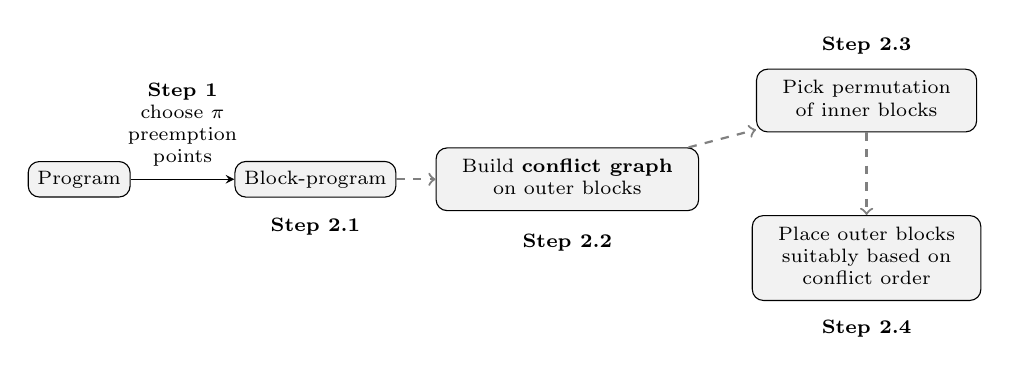
\begin{tikzpicture}[box/.style={rectangle, rounded corners, fill=gray!10, draw}]
  \node [box]  (a) at (0,0) {\scriptsize Program};
  \node [box] (b) at (3,0) {\scriptsize Block-program};
  \node [box] (c) at (6.2,0) {\scriptsize \begin{tabular}{c} Build \textbf{conflict graph} \\ on outer blocks \end{tabular}};
  \node [box] (d) at (10,1) {\scriptsize \begin{tabular}{c} Pick permutation \\ of inner blocks \end{tabular}};
  \node [box] (e) at (10,-1) {\scriptsize \begin{tabular}{c} Place outer blocks \\ suitably based on \\ conflict order \end{tabular}};
 
  

  \begin{scope}[->]
   \draw [>=stealth] (a) to node [above] {\scriptsize \begin{tabular}{c} \textbf{Step 1} \\ choose $\pi$ \\  preemption  \\ points \end{tabular}} (b);
   \draw [thick, dashed, gray] (b) to (c);
   \draw [thick, dashed, gray] (c) to (d);
   \draw [thick, dashed, gray] (d) to (e);
  \end{scope}

  \node at (3, -0.6) {\scriptsize \textbf{Step 2.1}};
  \node at (6.2, -0.8) {\scriptsize \textbf{Step 2.2}};
  \node at (10, 1.7) {\scriptsize \textbf{Step 2.3}};
  \node at (10, -1.9) {\scriptsize \textbf{Step 2.4}};
\end{tikzpicture}
\caption{Schema for the algorithm for \onewriter\ programs}
\label{fig:schema-one-writer}
 \end{figure}

\subsubsection*{Step 2.1. Partition the program $\program$ into Blocks : Block Programs}

A subset of events $\points \subseteq \eventset$ represents \emph{preemption points} if no event in $\points$ is the last event of its thread. Assume we have chosen a specific set $\points$ of preemption points. Note that when $\pi=0$, $\points$ is the emptyset.


Let $c^\points_i \ge 0$ be the number of events of thread $i$ in $\points$. 
We will omit the superscript and simply write $c_i$ when $\points$ is clear from the context. Furthermore,  $\sum_{i} c_i \le \pp$. Each thread $S_i$ can then be divided into blocks, based on the events of $S_i$ that are in $\points$, as explained next.


Consider thread $S_i$ as 

 $S_i = a_1 a_2 \dots a_m$.

Assume we guess events $a_{j_1}, a_{j_2}, a_{j_3}$ with $1 \le j_1 < j_2 < j_3 < m$ to be the events after which preemptions occur (in general, we guess $c_i$ events in thread $S_i$; we have taken $c_i = 3$ just as an example). This divides the thread into four blocks:
\begin{align*}
b^i_1: a_1 \dots a_{j_1} \qquad b^i_2: a_{j_1 + 1} \cdots a_{j_2} \qquad b^i_3: a_{j_2 + 1} \cdots a_{j_3} \qquad b^i_4: a_{j_3 + 1} \cdots a_m
\end{align*}
Each block is a contiguous set of events of a thread, and in every interleaving where the preemption points for $S$ occur at $a_{j_1}, a_{j_2}, a_{j_3}$, the events within a block appear contiguously, and moreover no two consecutive blocks of a thread appear next to each other. 

We denote the thread $S_i$ partitioned into blocks as $S_i^\points$. 
\begin{align*}
    \thread^\points_i = b^i_1 \cdot b^i_2 \cdots b^i_{c_i + 1}
\end{align*}
where each block $b^i_j$ is a contiguous sequence of events of $\thread_i$ ending in a preeemption point, as explained above. We call $\thread^\points_i$ as a \emph{block-thread}, and the set of block-threads $\thread^\points_1, \thread^\points_2, \dots, \thread^\points_k$ a \emph{block-program}, which we denote by $\program^\points$.

\begin{example}\label{eg:block-program}
In Figure~\ref{fig-onewriter-example} if $\points_1=\{(1:w(x,1)), (2:r(x,2))\}$ be the preemption points, then the block-program w.r.t. $\points_1$ would look as follows: 
\begin{alignat*}{2}
    \thread^{\points_1}_1 &=b^1_1\cdot b_2^1 &&=(1:w(x,1)) ~\cdot~ (1:w(x,2))(1:r(y,1))\\
     \thread^{\points_1}_2 
     &= b^2_1\cdot b_2^2 &&=(2:r(x,2)) ~\cdot~ (2:w(y,1))\\
      \thread^{\points_1}_3 &=b^3_1 &&=(3:r(x,1))
\end{alignat*}
where the first thread $\thread^{\points_1}_1$ is partitioned as  $b_1^1=(1:w(x,1))$, $b_2^1=(1:w(x,2))(1:r(y,1))$, and similarly for the other threads. 

Likewise, for the set $\points_2=\{(1:w(x,1)), (1:w(x,2))\}$ of preemption points, the block-program w.r.t. $\points_2$ would look as follows: 
\begin{alignat*}{2}\label{blockpartition}
    \thread^{\points_2}_1 &= b^1_1\cdot b_2^1\cdot b_3^1 &&=(1:w(x,1)) ~\cdot~(1:w(x,2))~\cdot~ (1:r(y,1))\\
     \thread^{\points_2}_2 
     &=b_1^2 &&=(2:r(x,2))(2:(w(y,1)))\\
      \thread^{\points_2}_3 &=b_1^3 &&= (3:r(x,1))
\end{alignat*}
Finally, for the set $\points_3=\emptyset$, $\thread^{\points_3}_1{=} b^1_1 {=} \thread_1$,  
$\thread^{\points_3}_2{=} b^2_1 {=} \thread_2$ and $\thread^{\points_3}_3{=} b^3_1 {=} \thread_3$ consist of a single block each.
\end{example}

A better illustration is given in right side of Figure~\ref{fig:example-algo} 
\subsubsection*{Sequential Consistency for Block Programs} We extrapolate the notion of sequential consistency in a natural way to the obtained block-program. A partial interleaving $\sigma^\points$ of $\program^\points$ is sequentially consistent if the partial interleaving $\sigma$ of the original program $\program$ obtained by expanding each block of $\sigma^\points$ into the contiguous sequence of events that it represents, is sequentially consistent. 

\begin{example}\label{eg:sc-for-block-programs}
Consider the program in Figure~\ref{fig-onewriter-example}. Let us call it $\program$. Then if we choose the set of preemption points $\points_1$ as in Example~\ref{eg:block-program}, $\sigma^{\points_1}=b^1_1\cdot b^3_1 \cdot b_1^2\cdot b_2^1\cdot b_2^2 $ is an interleaving for the block-program $\program^{\points_1}$. Note that this is not sequentially consistent as the last write on $x$ before $\rd(x,2)$ in $\sigma^{\points_1}$ is $\wt(x,1)$, which conflicts with $\rd(x,2)$. 
 Hence $\rd(x,2)$ has no write to read from.  
An example of a sequentially consistent interleaving of blocks from $\program^{\points_2}$ is: $\sigma^{\points_2}=b_1^1\cdot b_1^3\cdot b_2^1\cdot b_1^2\cdot b_3^1$.
\end{example}


\begin{figure}[t]
 \centering
 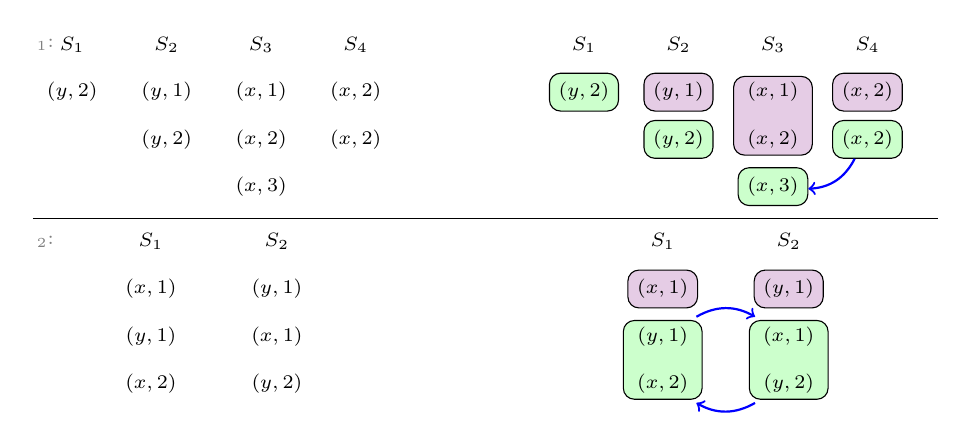
\begin{tikzpicture}
\begin{scope}
 \node at (0,0) {\scriptsize $S_1$};
 \node at (0,-0.6) {\scriptsize $\rd(y,2)$};
 \node at (1.2, 0) {\scriptsize $S_2$};
 \node at (1.2, -0.6) {\scriptsize $\wt(y,1)$};
 \node at (1.2, -1.2) {\scriptsize $\wt(y,2)$};
 \node at (2.4, 0) {\scriptsize $S_3$};
 \node at (2.4, -0.6) {\scriptsize $\wt(x,1)$};
 \node at (2.4, -1.2) {\scriptsize $\wt(x,2)$};
 \node at (2.4, -1.8) {\scriptsize $\wt(x,3)$};
 \node at (3.6, 0) {\scriptsize $S_4$};
 \node at (3.6, -0.6) {\scriptsize $\rd(x, 2)$};
 \node at (3.6, -1.2) {\scriptsize $\rd(x, 2)$};
\end{scope}

\begin{scope}[xshift=6.5cm, outer/.style={rectangle, rounded corners, fill=green!20, draw}, inner/.style={rectangle, rounded corners, fill=violet!20, draw}]
\node at (0,0) {\scriptsize $S_1$};
 \node [outer] at (0,-0.6) {\scriptsize $\rd(y,2)$};
 \node at (1.2, 0) {\scriptsize $S_2$};
 \node [inner] at (1.2, -0.6) {\scriptsize $\wt(y,1)$};
 \node [outer] at (1.2, -1.2) {\scriptsize $\wt(y,2)$};
 \node at (2.4, 0) {\scriptsize $S_3$};
 \draw [rounded corners, fill=violet!20] (1.9, -0.4) rectangle (2.9, -1.4);
 \node  at (2.4, -0.6) {\scriptsize $\wt(x,1)$};
 \node  at (2.4, -1.2) {\scriptsize $\wt(x,2)$};
 \node [outer] (b) at (2.4, -1.8) {\scriptsize $\wt(x,3)$};
 \node at (3.6, 0) {\scriptsize $S_4$};
 \node [inner] at (3.6, -0.6) {\scriptsize $\rd(x, 2)$};
 \node [outer] (a) at (3.6, -1.2) {\scriptsize $\rd(x, 2)$};
\end{scope}

\draw [->, thick, blue] (a) to [bend left] (b);

\draw (-0.5,-2.2) -- (11,-2.2);

%\node at (1.8, -2.2) {\scriptsize $\program_1$};
\node [left, thick, gray] at (-0.1, 0) {\scriptsize $\program_1$:};
\node [left, thick, gray] at (-0.1, -2.5) {\scriptsize $\program_2$:};

\begin{scope}[yshift=-2.5cm]
\node at (1, 0) {\scriptsize $S_1$};
\node at (1, -0.6) {\scriptsize $\wt(x,1)$};
\node at (1, -1.2) {\scriptsize $\rd(y,1)$};
\node at (1, -1.8) {\scriptsize $\wt(x,2)$};

\node at (2.6, 0) {\scriptsize $S_2$};
\node at (2.6, -0.6) {\scriptsize $\wt(y,1)$};
\node at (2.6, -1.2) {\scriptsize $\rd(x,1)$};
\node at (2.6, -1.8) {\scriptsize $\wt(y,2)$};

%\node at (1.8, -2.2) {\scriptsize $\program_2$};
\end{scope}

\begin{scope}[xshift = 6.5cm, yshift=-2.5cm, outer/.style={rectangle, rounded corners, fill=green!20, draw}, inner/.style={rectangle, rounded corners, fill=violet!20, draw}]
\node at (1, 0) {\scriptsize $S_1$};
\node [inner] at (1, -0.6) {\scriptsize $\wt(x,1)$};
\draw [rounded corners, fill = green!20] (0.5, -1) rectangle (1.5, -2);
\node (c) at (1, -1.2) {\scriptsize $\rd(y,1)$};
\node (e) at (1, -1.8) {\scriptsize $\wt(x,2)$};

\node at (2.6, 0) {\scriptsize $S_2$};
\node [inner] at (2.6, -0.6) {\scriptsize $\wt(y,1)$};
\draw [rounded corners, fill = green!20] (2.1, -1) rectangle (3.1, -2);
\node (d) at (2.6, -1.2) {\scriptsize $\rd(x,1)$};
\node (f) at (2.6, -1.8) {\scriptsize $\wt(y,2)$};

\draw [thick, blue, ->] (c) to [bend left] (d);
\draw [thick, blue, ->] (f) to [bend left] (e);
\end{scope}

\end{tikzpicture}
\caption{Programs $\program_1$ and $\program_2$ on the left, their corresponding block-programs on the right w.r.t. chosen preemption points. Inner blocks are coloured in violet, and outer blocks in green. The blue edges denote edges in the conflict graph of the outer nodes.}
\label{fig:example-algo}
\end{figure}

\begin{figure}[t]
\centering
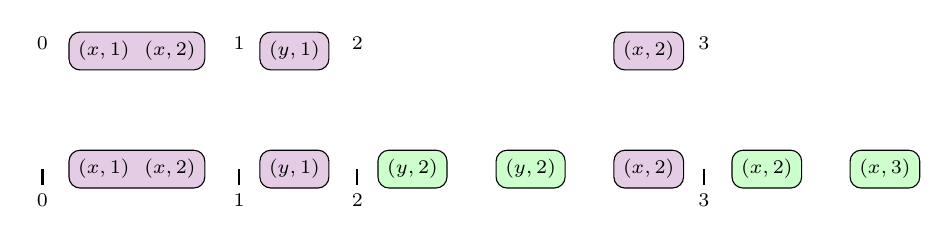
\begin{tikzpicture}[outer/.style={rectangle, rounded corners, fill=green!20, draw}, inner/.style={rectangle, rounded corners, fill=violet!20, draw}]

 \node [inner] (a1) at (0,1.5) {\scriptsize $\wt(x,1)~~\wt(x,2)$};
 % \draw [thick] (-1.2, 2) -- (-1.2, -0.2);
  \node at (-1.2, 1.6) {\scriptsize $0$};
  %\node at (0,-0.6) {\scriptsize $\wt(x,2)$};
  
  
  \node [inner] (b1) at (2,1.5) {\scriptsize $\wt(y,1)$};
%\draw [thick] (1.3, 0) -- (1.3, -0.2);
  \node at (1.3, 1.6) {\scriptsize $1$};

 % \draw [thick] (2.8, 0) -- (2.8, -0.2);
  \node at (2.8, 1.6) {\scriptsize $2$};

  \node [inner] (c1) at (6.5,1.5) {\scriptsize $\rd(x, 2)$};
  %\draw [thick] (7.2, 0) -- (7.2, -0.2);
  \node at (7.2, 1.6) {\scriptsize $3$};

  %\node [outer] at (3.5, 0) {\scriptsize $\wt(y, 2)$};
  %\node [outer] at (5, 0) {\scriptsize $\rd(y, 2)$};
  %\node [outer] at (8, 0) {\scriptsize $\rd(x,2)$};
  %\node [outer] at (9.5, 0) {\scriptsize $\wt(x,3)$};


  %\node [rectangle, rounded corners, fill=red!20, minimum size=1cm, draw] (a) at (0,-0.3) {};
  \node [inner] (a) at (0,0) {\scriptsize $\wt(x,1)~~\wt(x,2)$};
  \draw [thick] (-1.2, 0) -- (-1.2, -0.2);
  \node at (-1.2, -0.4) {\scriptsize $0$};
  %\node at (0,-0.6) {\scriptsize $\wt(x,2)$};
  
  
  \node [inner] (b) at (2,0) {\scriptsize $\wt(y,1)$};
\draw [thick] (1.3, 0) -- (1.3, -0.2);
  \node at (1.3, -0.4) {\scriptsize $1$};

  \draw [thick] (2.8, 0) -- (2.8, -0.2);
  \node at (2.8, -0.4) {\scriptsize $2$};

  \node [inner] (c) at (6.5,0) {\scriptsize $\rd(x, 2)$};
  \draw [thick] (7.2, 0) -- (7.2, -0.2);
  \node at (7.2, -0.4) {\scriptsize $3$};

  \node [outer] at (3.5, 0) {\scriptsize $\wt(y, 2)$};
  \node [outer] at (5, 0) {\scriptsize $\rd(y, 2)$};
  \node [outer] at (8, 0) {\scriptsize $\rd(x,2)$};
  \node [outer] at (9.5, 0) {\scriptsize $\wt(x,3)$};

  
\end{tikzpicture}
\caption{A permutation of inner blocks (above), and an interleaving obtained by 
inserting outer blocks at appropriate positions (below).}
\label{fig:example-algo-final-step}
\end{figure}


Thus,  there is a direct correspondence between interleavings of $\program$ and interleavings of a block-program $\program^\points$. When consecutive blocks within a thread do not appear together in an interleaving, then, it represents an interleaving of $\program$ where the preemptions occur exactly at $\points$.  We state this observation in the following lemma, whose proof follows directly from the definition of block-programs.


\begin{lemma}
Let $\points$ be a set of preemption points of $\program$. Then, $\program$ has a sequentially consistent interleaving where the preemptions occur at $\points$, iff the block-program $\program^{\points}$ has a sequentially consistent interleaving where no two consecutive blocks come from the same thread. 
\end{lemma}

The question therefore boils down to checking whether there is a sequentially consistent interleaving of $\program^{\points}$.

\noindent{\bf{Finding a sequentially consistent interleaving of a block-program}}.  
Recall that each thread has been divided into $c_i + 1$ blocks. A naive solution would be to enumerate all possible orderings of the $\sum_i (c_i + 1)$ blocks satisfying the program order and verify sequential consistency of each of them. However:
\begin{equation} 
  \sum_i (c_i + 1) = \sum_i c_i + \sum_i 1 \le \pp + k  \label{eq:naive} 
\end{equation} 
This only gives a complexity bounded by $(\pp + k)!$ which is not polynomial-time  when $\pp$ is the only fixed parameter.
Therefore, we propose a different procedure. 

\paragraph*{Dividing the block program into inner blocks and outer blocks.} Suppose $\program^{\points}$ is a block-program defined on the set of preemption points $\points$. We call the last block of any thread in $\program^{\points}$ as outer block and all other non-last blocks as inner blocks. In Figure~\ref{fig:example-algo}, all the violet blocks are inner blocks while the green blocks are outer blocks. As each inner block ends with a preemption point in $\points$, there are total $\pp$ inner blocks. Then the total number of outer blocks is $k$. We then  do a pre-processing that would add some ordering among the outer blocks of $\program^{\points}$ and discard the chosen set of preemptions $\points$ immediately if a cycle is found. 



\subsubsection*{Step 2.2. Conflict graph analysis on outer blocks}

By the end of Step 2.2, we have now identified the inner blocks and the outer blocks of $\program^{\points}$. 

We say the block $b_w$ conflicts block $b_r$ if (1) they belong to different threads, (2) there is a variable $x$ such that last write on $x$ in $b_w$ is in conflict with some read on $x$ in $b_r$. Then we order them as $b_r \to b_w$. Now look at the set of all outer blocks of $\program^{\points}$. For each outer block $b_w$, find if it is in conflict with some other outer block $b_r$. If yes, put the the order of conflict $b_r \to b_w$. This says that in any interleaving, $b_r$ appears before $b_w$. As $b_w$ is the last block of its thread, if $b_w$ writes to $x$ and is in conflict with $b_r$, $b_w$ cannot be executed before $b_r$. The blue edges in Figure~\ref{fig:example-algo} represents conflict order among the outer blocks. 

We can construct a conflict graph $G^{\program
^{\points}}$ as follows: For each outer block there is a node in $G$. For each outer block $b_w$ if it conflicts some other outer block $b_r$, we put the edge $b_r \to b_w$. In Figure~\ref{fig:example-algo},  for $\program_1$, $\rd(x, 2)$ should appear before $\wt(x, 3)$; for $\program_2$, there are two induced orderings due to the different variables $x$ and $y$.

If there is a cycle in the conflict graph (as in $\program_2$) we declare that there exists no SC interleaving for the chosen set of preemptions $\points$. If there is no such cycle (for instance, $\program_1$), we move to Step 2.3. 

\paragraph*{Complexity}: For each of the $k$ outer blocks we check if it conflicts some other outer block. To do this, given an outer block $b$, for every variable $x$ that the block writes, we check if the last write on $x$ in $b$ is in conflict with any read of other outer blocks. Thus constructing the graph takes $\mathcal{O}(n\cdot k)$ time. Next we check for a cycle. This takes not more than $\mathcal{O}(k^2)$ time. As $k< n$, Step 2.2 would take $\mathcal{O}(n\cdot k)$ time to run. 

\subsubsection*{Step 2.3. Placing outer blocks in a Permutation of Inner Blocks.}

Consider all possible permutations of the inner blocks. Since there are at most $\pp$ in number, there are at most $\pp!$ permutations. The goal is to check if we can place the $k$ outer blocks between these inner blocks so as to obtain an SC interleaving. In Figure~\ref{fig:example-algo-final-step}, the top illustrates an ordering for inner blocks.  We have also marked the positions around the inner blocks (in the figure, they are marked as $0, 1, 2$ and $3$). The outer blocks need to be placed appropriately.

\subsubsection*{Step 2.4. Placing the outer blocks respecting conflict}

After the conflict analysis returns no cycle for the conflict graph $G^{\program
^{\points}}$, in Step 2.3 we choose a permutation $p$ of the inner blocks. On each of these $\pp!$ permutations we now call Algorithm~\ref{pseudocode:vscp-interleaving}. This is the final step which returns an SC interleaving of the blocks of $\program^{\points}$. For this section $\program$ refers to $\program^{\points}$ and $G$ refers to $G{\program
^{\points}}$. We omit the superscript of the notations.



\begin{algorithm}[h]
\caption{Module to obtain an $\scmm$-consistent block interleaving from a given block program $\program$}\label{pseudocode:vscp-interleaving}

\Input{A block-program $\program$ of a $\onewriter$ program, a permutation $\sigma=\{b_1,b_2,\cdots,b_{\pp}\}$  on inner blocks and an acyclic conflict graph $G$ on the outer blocks}
\Output{an $\scmm$ consistent interleaving of blocks}
\smallskip

\Fn{CheckSC($\program$, $\sigma$, $G$)}{

    $G'=$ a linearization of $G$;
    
    $test=0$;
    
    $b'=\epsilon$;
    
    Add dummy block $b_{\pp+1}$ to $\sigma$;
    
    \For{$i\gets0$ \KwTo $\pp+1$}{\label{for-loop-outer}
        
        \While{there exists an outer block which is enabled}{\label{While-loop}
        
        Choose the earliest enabled block $b$ in $G'$;
        
        \For{$j\gets i+1$ \KwTo $\pp$}{\label{For-loop-iner}
                \If{$b$ conflicts $b_j$} {\label{if-conflict}
                
                test$=1$; 
                
                \Break;}
            
            }
            
            \If{$test=0$}{
            
            Place $b$ between $b'$ and $b_{i+1}$ in $\sigma$;
            
            $b'=b$;
            
            Remove $b$ from $G'$;}
        
        }
        
        $b'=b_{i+1}$;
        

    }
    
    \If{$\sigma$ is $\scmm$-consistent and $G'$ is empty}{\Return 1;}
}


\end{algorithm}

Algorithm~\ref{pseudocode:vscp-interleaving} describes Step 2.4 of the polynomial time algorithm for \vscp. The input is a block-program of a single writer system  divided into inner and outer blocks, a permutation of the inner blocks $\sigma$ and a conflict graph $G$ on the outer blocks. Recall that outer blocks are the last blocks of each block sequence. It takes a linearization $G'$ of $G$ and uses it to place the outer blocks in their correct position in $\sigma$ so that the resulting interleaving is $\scmm$-consistent. 

Description: The algorithm~\ref{pseudocode:vscp-interleaving} chooses a linearization $G'$ of $G$. For each position between the consecutive inner block in $\sigma$, beginning from the left to $b_1$, the algorithm places all enabled outer blocks such that the conflict order of $G$ is satisfied. Note that any outer  block $b$ is enabled at some position only if (1) all blocks above it in its thread are already in sigma before the currently considered position (2) if the last block before the current position is $b'$ and the prefix of $\sigma$ upto $b'$ is $\sigma'$, then $\sigma'\cdot b$ should be $\scmm$-consistent. The variable $b'$ captures the last position in $\sigma$ where a block has been inserted. Moreover, $b$ should not conflict any inner block of $\sigma$ at any later position. This is captured by the condition of the \emph{If} statement in line~\ref{if-conflict}. At the end of the outer for-loop, if no more outer blocks remain to be inserted in $\sigma$, and the resulting interleaving $\sigma$ is $\scmm$-consistent, return 1.

Continuing with our running example $\program_1$ in Figure~\ref{fig:example-algo-final-step}, at position $0$, none of the outer blocks is enabled: the outer block in $S_1$ requires a writing source, and the outer blocks in the other threads cannot be scheduled unless earlier blocks in the program order are completed. So we move to position $1$. At position $1$, the outer block $\wt(x, 3)$ of $S_3$ is enabled since the inner block $\wt(x,1).\wt(x,2)$ of $S_3$ 
appears already.  However, we cannot place it at position 1 for two reasons: firstly, it conflicts the inner block $\rd(x, 2)$ that appears in front of position 3 to the right; and secondly there is an outer $\rd(x,2)$ block which needs to appear before $\wt(x, 3)$ according to the ordering induced by the conflict. Therefore, we do not place it at position $1$ and move on to position $2$. At position $2$, the enabled outer blocks are $\wt(y, 2)$ and $\wt(x, 3)$. We place $\wt(y, 2)$ and not $\wt(x, 3)$ for the same reasons as above. Once $\wt(y, 2)$ is placed, the outer block $\rd(y, 2)$ is also enabled. We place it and move on to position $3$. Here, both $\wt(x, 3)$ and the outer block $\rd(x, 2)$ are enabled. Based on the conflict ordering, we place $\rd(x, 2)$ followed by $\wt(x, 3)$. 

Thus, at each position in a given permutation of inner blocks,
 we find the enabled outer blocks among the ones yet to be scheduled, and  place them according to the ordering induced by the conflicts. Moreover, we place an outer block at a position only if it does not conflict any inner block appearing later. Placing an outer block at a position may enable more outer blocks. We finish with the position only when there are no more outer blocks that can be placed at that position.  
 
\noindent{\bf{A final check}.} If some outer blocks cannot be placed, we conclude that an SC interleaving is not possible for the chosen permutation of the inner blocks. Otherwise, all outer blocks have been placed. Still, we need to do a final check to ensure SC. This is because, we had chosen an arbitrary permutation of inner blocks. There could be reads in inner blocks with no writing source, even after the placement of outer blocks; and secondly there could be reads in inner blocks which contradict later reads in an inner block, even after the outer blocks are all placed. If the interleaving satisfies SC, we are done. Else, we move to another permutation of inner blocks, until we exhaust all of them.


Complexity: Finding a linearization of $G$ requires $O(k^2)$ time. Note that the for-loop in line~\ref{for-loop-outer} runs $\mathcal{O}(\pp)$ times while testing the while loop condition takes $\mathcal{O}(n)$ time units. The inner for-loop takes no more than $\mathcal{O}(n)$ time to run. Any other statements inside the while-loop does not take more than $\mathcal{O}(n)$ time. The while-loop can atmost run $k$ times as there are atmost $k$ outer  threads. Thus the total complexity of the procedure is  $\mathcal{O}(\pp nk+k^2)=\mathcal{O}(\pp nk)$ as $k<n$.  


\begin{theorem}
 A block program $\program$ has an $\scmm$-consistent interleaving of all its blocks if and only if the  algorithm~\ref{pseudocode:vscp-interleaving} returns 1 for some permutation of the inner blocks of $\program$.
\end{theorem}

\begin{proof}
$(\Leftarrow)$ This direction is direct. Whenever the algorithm returns 1 for some permutation of the inner blocks of $\program$, there is an $\scmm$-consistent execution of $\program$. This is because we insert any outer block at some position if and only if it does not conflict any inner block later to that position and it is enabled there. Also any conflict between the outer blocks is respected while the placing the outer blocks. This is supported by the fact that only the earliest enabled block of $G'$, a linearization of the conflict graph $G$, is chosen at each iteration of the while-loop in algorithm~\ref{pseudocode:vscp-interleaving}. Also the last check for $\scmm$-consistency strengthens our claim.

 $(\Rightarrow)$ Let $\program$ has an $\scmm$ consistent interleaving $\sigma$  for some permutation of its inner block $p$. We shall show that with $p$ as an input, the algorithm will return 1. Note that there must be no conflicting cycle among the outer blocks or else $\prog$ wouldn't have any $\scmm$-consistent execution. Let us define a few auxiliary notions. 
 
 Let $P=\{b_1,b_2,\cdots,b_{\pp}\}$ be a permutations of the $\pp$ inner blocks of $\program$. $S_P$ be the set of all $\scmm$-consistent interleavings of $\program$ with order of inner blocks $p$. 
 Let $\sigma_1,\sigma_2\in S_P$. We say $\sigma^b$ is a prefix of $\sigma$ upto block $b$. Then we say $\sigma_1<\sigma_2$ if $\sigma_1^{b}$ has equal or more number of blocks than $\sigma_2^{b}$ for all blocks $b$ in $p$. Then there exists an interleaving $\sigma'$ such that $\sigma'<\sigma$ for all $\sigma\in S_P$. We call such an interleaving a `nice' interleaving. We shall show that a nice interleaving can be generated by our algorithm. 

 Let $R$ be the set of all interleavings obtained from our algorithm on $p$. 
Let $b$ be the first block of $\sigma$. If $b$ is an inner block, the prefix of $\sigma$ upto $b$ matches all interleavings of $\sigma$. Else if $b$ is an outer block, $b$ must be enabled at the first iteration of the while-loop in algorithm~\ref{pseudocode:vscp-interleaving}. As $b$ is an outer block, it must not conflict any $inner$ block of $p$ or else it would have been not placed as the first block in $\sigma$. Note that this could be said only because we are dealing with $\onewriter$. For multiple writers there would be more outer blocks that can conflict some inner blocks on the same variable as $b$. Thus $b$'s place would not be determined. 

Let $\sigma^b$ be the longest prefix that matches some interleaving in $R$. Surely, Let us look at $\sigma^b.b'$. If $b'$ is an inner block, there must not be any enabled outer block that does not conflict with the inner blocks not included in $\sigma^b$. Otherwise, $\sigma^b$ would not be `nice'. There would be an interleaving $\sigma'$ in $R$ such that $\sigma'<\sigma$. But then there must be an interleaving in $R$ with prefix $\sigma^b.b'$. 

On the other hand if $b'$ is an outer block, (1) $\sigma^b.b'$ must be $\scmm$-consistent (2) $b'$ cannot conflict any block not in $\sigma^b$. Our algorithm then is free to choose $b'$ after $\sigma^b$. Hence $\sigma^b.b'$ must be the prefix of some interleaving in $R$. By induction, our claim follows.
\end{proof}
 
\subsubsection*{Why the conflict analysis does not work for inner blocks and \twowriter\ programs?}

Let us once again consider the $\program_1$ example from Figure~\ref{fig:example-algo}. There $\rd(x,2)$ is in conflict with $\wt(x,3)$. If $\wt(x, 3)$ is not an outer block, it may still be possible to have an interleaving where $\wt(x,3)$ appears before $\rd(x,2)$ as long as there is a later block below $\wt(x,3)$ with a matching $\wt(x,2)$. So, there is no forced order. A similar phenomenon happens for \twowriter\ systems too. We cannot force an order between two blocks just because there is conflict in the read and write. This leads to a blow-up in the permutations. Infact the next chapter indicates that VSC$^\pp$-problem is $\np$-Complete for programs with multiple writers even with $\pp = 0$. This exemplifies the crucial advantage of the conflict analysis in \onewriter\ systems.


  





%Now why would the conflict analysis not work for more than one threads? Try to understand why it did work for \onewriter{}. 
%In \onewriter{} programs all writes on the same variable are in the same thread. Hence,  in any  block program, there is only one outer block that writes to a particular variable. For a given block program and for a given permutation of inner blocks, we just need to seek the appropriate position of the reads, with the help of the conflict graph. But if there are multiple outer blocks writing to the same variable, the conflict graph may not help. We do not know the order among the writer blocks now. Example, if there are three outer blocks representing only the events $\wt(x,d)$, $\wt(x,d')$ and $\rd(x,d'')$ respectively,  then $\rd(x,d'')$ is in conflict with both of them, but how do we order $\wt(x,d)$ and $\wt(x,d')$?

%%%%%%%%%%%%%%%%%
%%%%%%%%%%%%%%%%%
%%%%%%%%%%%%%%%%%

\endinput
